
%-----------------------------------------------------------------------------------
%	PACKAGES AND OTHER DOCUMENT CONFIGURATIONS
%----------------------------------------------------------------------------------



\documentclass[11pt]{article}

\usepackage[top=2cm, bottom=3cm, left=2cm, right=2cm]{geometry}

\setlength{\parindent}{0in}

\newcommand{\Var}{\mathrm{Var}}

\newcommand{\Cov}{\mathrm{Cov}}

\newcommand{\plim}{\rightarrow_{p}}

\usepackage{amsmath, amsfonts}
\usepackage{graphicx}
\usepackage{pdfpages}
\usepackage{bm}
\usepackage{listings}

% Expectation symbol
\newcommand{\E}{\mathrm{E}}
\newcommand{\V}{\mathrm{V}}

%----------------------------------------------------------------------------------
%	TITLE AND AUTHOR(S)
%----------------------------------------------------------------------------------

\title{PubPol 713 Assignment 1} % The article title


\author{Nathan Mather} % The article author(s) 

\date{\today} % An optional date to appear under the author(s)


%----------------------------------------------------------------------------------
\begin{document}
	
%------------------------------------------------------------------------------
%	TABLE OF CONTENTS & LISTS OF FIGURES AND TABLES
%------------------------------------------------------------------------------
\maketitle % Print the title/author/date block

\setcounter{tocdepth}{2} % Set the depth of the table of contents to show sections and subsections only

%\tableofcontents % Print the table of contents

%-------------------------------------------------------------
% Question 1 
%-------------------------------------------------------------
\section{ Question 1}

\begin{center}
	\begin{tabular}{||c | c||} 
		\hline
		Variable & Meaning  \\ [0.5ex] 
		\hline\hline
		$EngShare_{jt}$ & Share of Majors that are Engineering for school j in a year t \\ 		
		\hline 
		$EngDiff_{jt}$ & school j has Price differentials in year t\\ 
		\hline
		$\delta_t$ & fixed effect for year t \\ 
		\hline
		$\lambda_t$ &  fixed effect for school j\\
		\hline
		$\epsilon_{jt}$ & Error Term \\
		\hline
		$EngDiff\_02_{jt}$ & school j has price differential in yeat t to t-2 \\
		\hline
		$EngDiff\_3plus_{jt}$ & School J has price differential in year t-3 or before \\[1ex] 
		\hline
	\end{tabular}
\end{center}


model (1):  \\ \\ 

$$
EngShare_{jt} = \beta_0 +  \beta_1  EngDiff_{jt} + \epsilon_{jt}  $$

For model (1) $\beta_1$ is the coefficient of interest and it measures the association of enacting an Engineering differential with the share of students majoring in engineering. 
\\ \\ 
model (2): \\ \\ 

$$
EngShare_{jt} = \beta_0 +  \beta_1  EngDiff_{jt} + \delta_t + \lambda_j + \epsilon_{jt}   $$

For model (2) $\beta_1$ is the coefficient of interest and it measures the association of enacting an Engineering differential with the share of students majoring in engineering while holding the impact of the year and the school constant. 
\\ \\ 
model (3): \\ \\ 
$$
EngShare_{jt} = \beta_0 +  \beta_1  EngDiff\_02_{jt} + \beta_2 EngDiff\_3plus_{jt} + \delta_t + \lambda_j + \epsilon_{jt}   $$

For Model (3) the coefficients of interest are $\beta_1$ and $\beta_2$. An engineering differential having been enacted in the last two years is associated with a $\beta_1$ increase in the share of students majoring in engineering. And engineering differential having been enacting 3 or more years earlier is associated with a $\beta_2$ increase in the share of students majoring in engineering. 
\\ \\
model (4): \\ \\ 

Model 4 has the same equation as model 3, but has a restricted sample. As Stange puts it this "restrict[s] the
analysis sample to include observations for treatment schools only within an eight year window; around the year differential pricing was enacted."




%-------------------------------------------------------------
% Question 2
%-------------------------------------------------------------
\section{Question 2}
The results of my replication are in Table 1 column (1) below. These results show the correlation between having an engineering differential and the share of students majoring in engineering. Having an engineering differential is associated with 5.9 percentage point increase in students majoring in engineering. Omitted variables include time shocks to major preference. for example, it may be that there is an increase in the share of students majoring in engineering due to rising pay for engineers. This would lead to fewer engineering majors before the policies and more after, but not as a result of the law.  

%-------------------------------------------------------------
% Question 3
%-------------------------------------------------------------
\section{Question 3}
the results are in Table 1 column (2) below. We have a significant negative relationship. So enacting an engineering differential is associated with a drop in the share of engineering students by 1 percentage point holding the year constant and the school constant. \\ \\ 

I expected the year fixed effects to have a bigger impact, but either one makes sense. To check this I ran the regression with only year fixed effects, model (2)a in table 1, and with only institution fixed effects, model (2)b in Table 1. The results suggest that I was wrong and institution fixed effects are playing a bigger role as the coefficient is more positive with only year fixed effects but is negative with only institution fixed effects. 


%-------------------------------------------------------------
% Question 4
%-------------------------------------------------------------
\section{Question 4}

Models 3 and 4 break up the impact of differential pricing into an immediate impact of the first year enacted and the following two years as well as a long term impact of 3 years after the policy or later. The results of both models suggest that there is an initial negative impact on engineering majors, and this impact grows over time. This makes sense as students that have already chosen their major are less likely to change majors as a result. Older students also have a lower cost for graduating with the major since they would, on average, have fewer years remaining in school. 


%-------------------------------------------------------------
% Question 5
%-------------------------------------------------------------
\section{Question 5}

This would lead to a positive bias in the estimates. This is because their is an omitted variable, region, that is correlated with both implementing a price differential and having higher engineering enrollment. Including dummies for the census divisions would solve this problem. This is model (5) in Table 1. It does not alter the results form model 4. 


\begin{center}
	
	\centering
	\LARGE{\textbf{Table 1}}\par\medskip
	
	\normalsize{\textbf{Replication Results }}\par\medskip
	\scalebox{1}{
		{
\def\sym#1{\ifmmode^{#1}\else\(^{#1}\)\fi}
\begin{tabular}{l*{7}{c}}
\hline\hline
            &\multicolumn{1}{c}{(1)}&\multicolumn{1}{c}{(2)}&\multicolumn{1}{c}{(2)a}&\multicolumn{1}{c}{(2)b}&\multicolumn{1}{c}{(3)}&\multicolumn{1}{c}{(4)}&\multicolumn{1}{c}{(5)}\\
\hline
engdiff     &      0.0588\sym{*}  &     -0.0105\sym{*}  &      0.0641\sym{*}  &     -0.0174\sym{**} &                     &                     &                     \\
            &    (0.0275)         &   (0.00521)         &    (0.0290)         &   (0.00532)         &                     &                     &                     \\
[1em]
engdiff\_02  &                     &                     &                     &                     &    -0.00437         &    -0.00426\sym{*}  &    -0.00426\sym{*}  \\
            &                     &                     &                     &                     &   (0.00402)         &   (0.00203)         &   (0.00203)         \\
[1em]
engdiff\_3plus&                     &                     &                     &                     &     -0.0171\sym{*}  &     -0.0111\sym{**} &     -0.0111\sym{**} \\
            &                     &                     &                     &                     &   (0.00730)         &   (0.00392)         &   (0.00392)         \\
[1em]
\_cons      &      0.0789\sym{***}&      0.0455\sym{***}&      0.0953\sym{***}&      0.0353\sym{***}&      0.0452\sym{***}&      0.0449\sym{***}&      0.0582\sym{***}\\
            &   (0.00864)         &   (0.00190)         &    (0.0102)         &  (2.85e-16)         &   (0.00190)         &   (0.00203)         &   (0.00203)         \\
\hline
\(N\)       &        2698         &        2698         &        2698         &        2698         &        2698         &        2304         &        2304         \\
\(R^{2}\)   &       0.027         &       0.979         &       0.033         &       0.977         &       0.979         &       0.978         &       0.978         \\
\hline\hline
\multicolumn{8}{l}{\footnotesize Standard errors in parentheses}\\
\multicolumn{8}{l}{\footnotesize \sym{*} \(p<0.05\), \sym{**} \(p<0.01\), \sym{***} \(p<0.001\)}\\
\end{tabular}
}

	}
\end{center}


%-------------------------------------------------------------
% Question 6
%-------------------------------------------------------------
\section{Question 6}

$$
EngShare_{jt} = \alpha_0 + \sum_{k=-3}^{k=4^+} \beta_k StartEngdiff_{j, t+k} +  \delta_t + \lambda_j + \epsilon_{jt}   $$
 
 just as in the paper, "$StartEngdiff_{j, t+k}$ indicates that institution j adopted differential pricing for engineering k years before t." \\ \\ 
 
 the $\beta_k$'s are the coefficients of interest. As in the paper they are "the change in share of degrees granted in engineering k years after the adoption of differential pricing relative to the omitted category (k = −4 or earlier)" holding the institution and year constant. I omit the vector of controls used in the paper as this provides a more direct comparison to the models run in the question above.  \\ \\ 
 

 %-------------------------------------------------------------
 % Question 7
 %-------------------------------------------------------------
 \section{Question 7}
 
 \begin{center}
 	
 	\centering
 	\textbf{Figure 2 Replication}\par\medskip
 	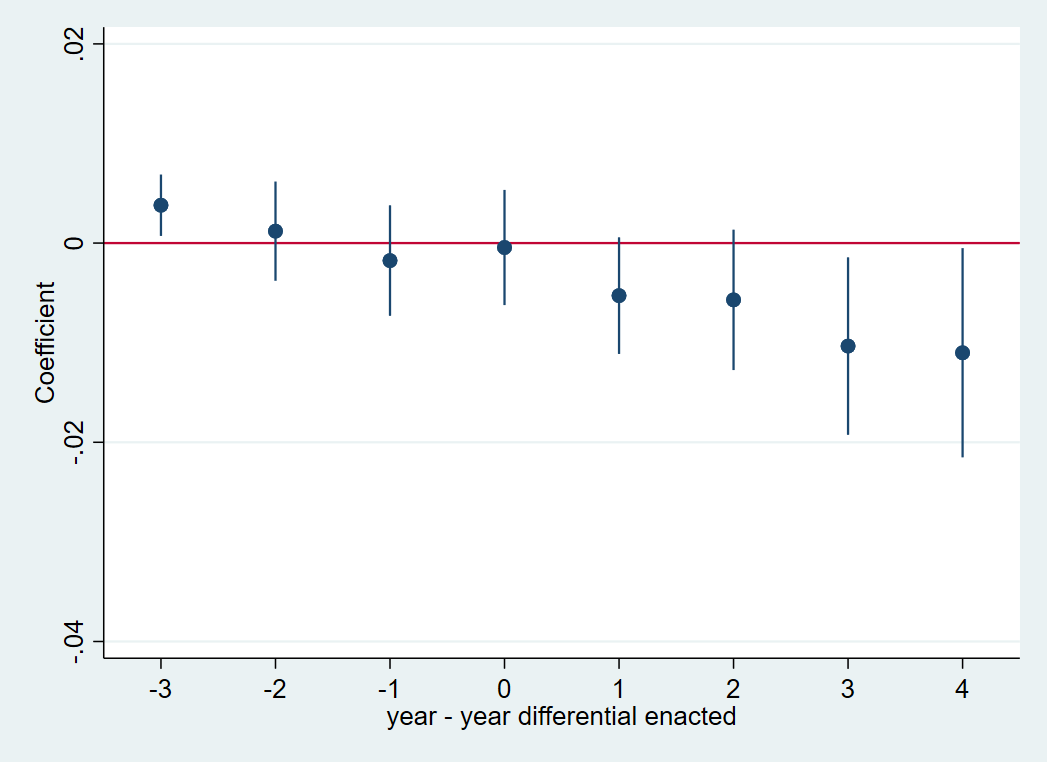
\includegraphics[width=1\linewidth]{ps1_figure_eng_share.png}
 \end{center}
 
 The coefficient on StartEngDiffpost3 is the association of having a price differential enacted for engineering three years prior relative to not having one in place for the next 4 years or more. 
 
 
  %-------------------------------------------------------------
 % Question 8
 %-------------------------------------------------------------
 \section{Question 8}
 
 If the difference in difference estimate is valid we should see a change in the coefficient at zero that persists. The Difference in difference assumes a discrete event where before is not treated and after is treated.
 \\ \\ 
 The assessment suggests that the difference in difference is probably a reasonable model.  we have coefficients around zero before the event and that are negative after. There appears to be another dip after 2 year so the specification in model 3 and 4 seems warranted. 
 
  %-------------------------------------------------------------
% Question 9
%-------------------------------------------------------------
\section{Question 9} 

The only difference in the interpretation is that now the effects are relative to a year before the differential policy was enacted rather than relative to being 4 or more years before the policy is enacted. The results of both regressions can be seen in table 2. We can see, for example, that the coefficient on StartEngDiffpre3 is 0.0038 when StartEngDiffpre4 is omitted and .00556 when StartEngDiffpre3 is omitted. This difference is the difference between StartEngDiffpre4 and StartEngDiffpre1, which can be seen by the coefficients of 0.00176 and -0.00176 respectively.
This is true of any set of dummy variables where on is omitted. The coefficients and interpretation change, but the result is the same. 
 
 \begin{center}
 	
 	\centering
 	\LARGE{\textbf{Table 2}}\par\medskip
 	
 	\normalsize{\textbf{Event study}}\par\medskip
 	\scalebox{1}{
 		{
\def\sym#1{\ifmmode^{#1}\else\(^{#1}\)\fi}
\begin{tabular}{l*{2}{c}}
\hline\hline
            &\multicolumn{1}{c}{(1)}&\multicolumn{1}{c}{(2)}\\
            &\multicolumn{1}{c}{eng\_share}&\multicolumn{1}{c}{eng\_share}\\
\hline
StartEngDiffpre4&                     &     0.00176         \\
            &                     &   (0.00281)         \\
[1em]
StartEngDiffpre3&     0.00380\sym{*}  &     0.00556\sym{*}  \\
            &   (0.00156)         &   (0.00228)         \\
[1em]
StartEngDiffpre2&     0.00120         &     0.00295         \\
            &   (0.00252)         &   (0.00209)         \\
[1em]
StartEngDiffpre1&    -0.00176         &                     \\
            &   (0.00281)         &                     \\
[1em]
StartEngDiffpost0&   -0.000444         &     0.00131         \\
            &   (0.00293)         &   (0.00168)         \\
[1em]
StartEngDiffpost1&    -0.00527         &    -0.00352         \\
            &   (0.00296)         &   (0.00235)         \\
[1em]
StartEngDiffpost2&    -0.00570         &    -0.00394         \\
            &   (0.00357)         &   (0.00276)         \\
[1em]
StartEngDiffpost3&     -0.0103\sym{*}  &    -0.00858\sym{**} \\
            &   (0.00451)         &   (0.00308)         \\
[1em]
StartEngDiffpost4plus&     -0.0110\sym{*}  &    -0.00925\sym{*}  \\
            &   (0.00531)         &   (0.00378)         \\
[1em]
\_cons      &      0.0449\sym{***}&      0.0449\sym{***}\\
            &   (0.00204)         &   (0.00204)         \\
\hline
\(N\)       &        2304         &        2304         \\
\(R^{2}\)   &       0.978         &       0.978         \\
\hline\hline
\multicolumn{3}{l}{\footnotesize Standard errors in parentheses}\\
\multicolumn{3}{l}{\footnotesize \sym{*} \(p<0.05\), \sym{**} \(p<0.01\), \sym{***} \(p<0.001\)}\\
\end{tabular}
}

 	}
 \end{center}
 .\\
 \\
 \\
 \\\\
 \\
 \\
 
 
  \begin{center}
 	
 	\centering
 	\textbf{Event study with StartEngDiffpre1 omitted }\par\medskip
 	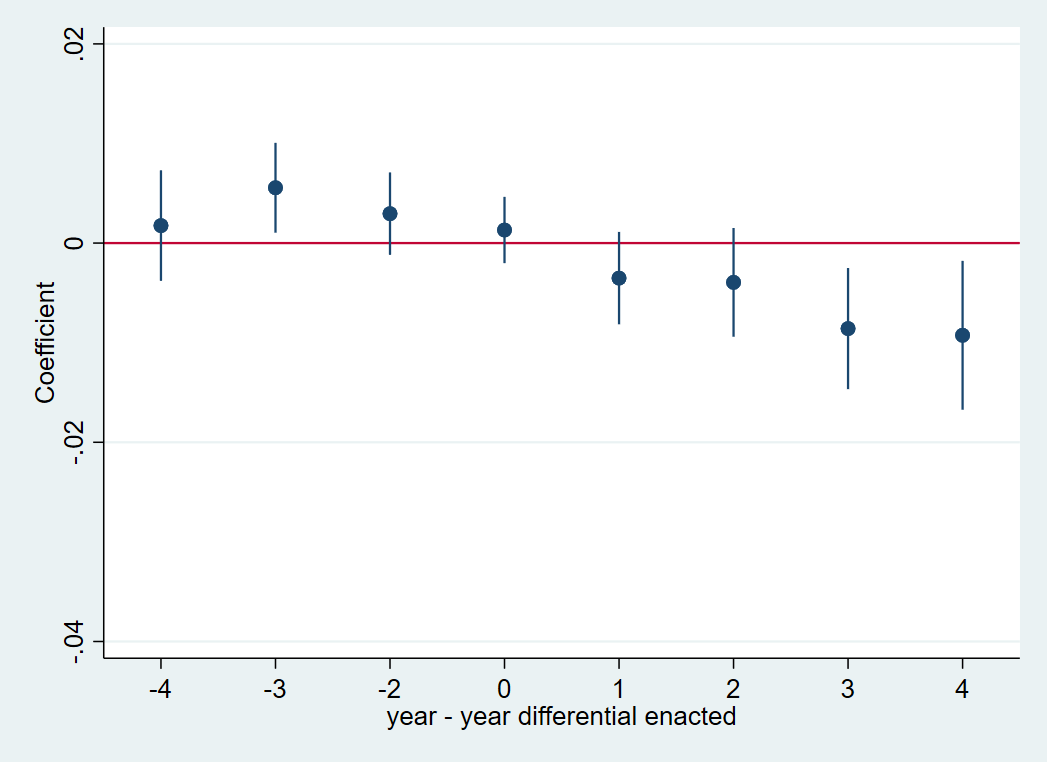
\includegraphics[width=1\linewidth]{ps1_figure_eng_share2.png}
 \end{center}
 
%------------------------------------------------
% end doc
%------------------------------------------------
\end{document}


